% This conference manuscript template is prepared for:   
% Kim Stockment, Conference Coordinator, Ray W. Herrick Laboratories, Purdue University, West Lafayette, IN, USA. 
% Latest revision = 2016-02-23 

\documentclass[10pt]{article}
% Miktex users: require l3 packages
%             : optional 3 packages
\usepackage{amssymb,amsmath,multicol,titlesec,apacite,booktabs,tabto,url, multirow, makecell, eurosym}
%\usepackage[round]{natbib}  
\usepackage{longtable}

\usepackage[hmargin = 1in, vmargin = 1in]{geometry}

\renewcommand{\refname}{References}
    
%\usepackage[MnSymbol]{mathspec}
%\setallmainfonts{Times New Roman}
% Mathspec requires the XeTeX compiler. 

\usepackage[parfill]{parskip}
\usepackage{graphicx}
\usepackage[font=bf]{caption}
\usepackage{siunitx}
\usepackage{changepage}  % allows to use adjustwidth
\usepackage{xcolor}

\usepackage{titlesec} 
%\titleformat{command}[shape]{format}{label}{sep}{before}[after]
\titleformat{\section}[hang]{\fontsize{12pt}{1em}\selectfont \bfseries}{\thesection. }{0pt}{\centering \MakeUppercase}
\titleformat{\subsection}[hang]{\fontsize{11pt}{1em}\selectfont \bfseries}{\thesubsection}{5pt}{}
\titleformat{\subsubsection}[runin]{}{\thesubsubsection}{5pt}{} 
%\titlespacing{command}{left}{beforesep}{aftersep}[right]
\titlespacing{\section}{0pt}{10pt}{10pt}
\titlespacing{\subsection}{0pt}{10pt}{0pt}
\titlespacing{\subsubsection}{0pt}{10pt}{0pt}	
%\setlength{\bibsep}{3pt}
%\pagenumbering{\gobble}
%\setlength{\hyphenpenalty}{1000}
%\setlength{\exhyphenpenalty}{1000}

\usepackage{fancyhdr}
\pagestyle{fancy}
\fancyhead[R]{\fontsize{12pt}{1em}\selectfont {{\textbf{Page \thepage}}}}
\fancyhead[L]{}
\fancyfoot[C]{IBPSA Project 1, September 2019}
\renewcommand{\headrulewidth}{0pt} % Turn off the bar

\newcommand\thefontsize[1]{{#1 The current font size is: \f@size pt\par}}



% % % % % % % % % % % % % %  TITLE  % % % % % % % % % % % % % %

\title{MPC formulation description template}


\author{J\'an Drgo\v{n}a$^{1,2}$,  Iago Cupeiro Figueroa$^{1}$}
\date{ ${1}$ Department of Mechanical Engineering,  KU Leuven, Belgium \\
        {\tt\small \{jan.drgona,iago.cupeirofigueroa\}@kuleuven.be}  \\
            {${2}$ Pacific Northwest National Laboratory, Richland, WA, USA \\
        {\tt\small jan.drgona@pnnl.gov}} \\%
        \vspace{0.2cm}
    \today
}


\begin{document}
	
	\maketitle


\section*{ABSTRACT}

This document describes the MPC formulation template as used within the frame of the IBPSA Project 1.
The proposed template aims to uniformize all possible formulations for the different types of models and key performance indicators (KPIs) in consideration.
It has to be general.
To this end, we choose the control engineering notation as our starting point,
since it considers the formulation in a general way from an abstract point of view.
From here, we move to a formulation with physical meaning based on the specific characteristics of buildings.


%\section*{NOMENCLATURE}
%
%\begin{samepage}
%	$x$\tabto{1.0in}Vector of states	\\
%	$u$\tabto{1.0in}Vector of inputs	\\
%	$y$\tabto{1.0in}Vector of outputs\\	
%	$d$\tabto{1.0in}Vector of disturbances\ \\
%	$N$\tabto{1.0in}Prediction horizon
%	
%\end{samepage}
%\begin{samepage}
%	\textbf{Subscript}\\
%	$k$\tabto{1.0in}Considered time-step index
%\end{samepage}


\section{CONTROL ENGINEERING NOTATION}\label{sec:control_notation}

{\color{blue} 
We build up the control engineering notation based on a general building model structure presented in
Fig.~\ref{fig:Building_model}.
The set of abstract domain variables represents the states of a system $x$, the heat flows to a system $u$, the disturbances  $d$, the controlled variables  $y$,  the actuator variables  $y$, the additional measured variables $m$, and the reference signals $r$. }
\begin{figure}[!htbp]
\centering
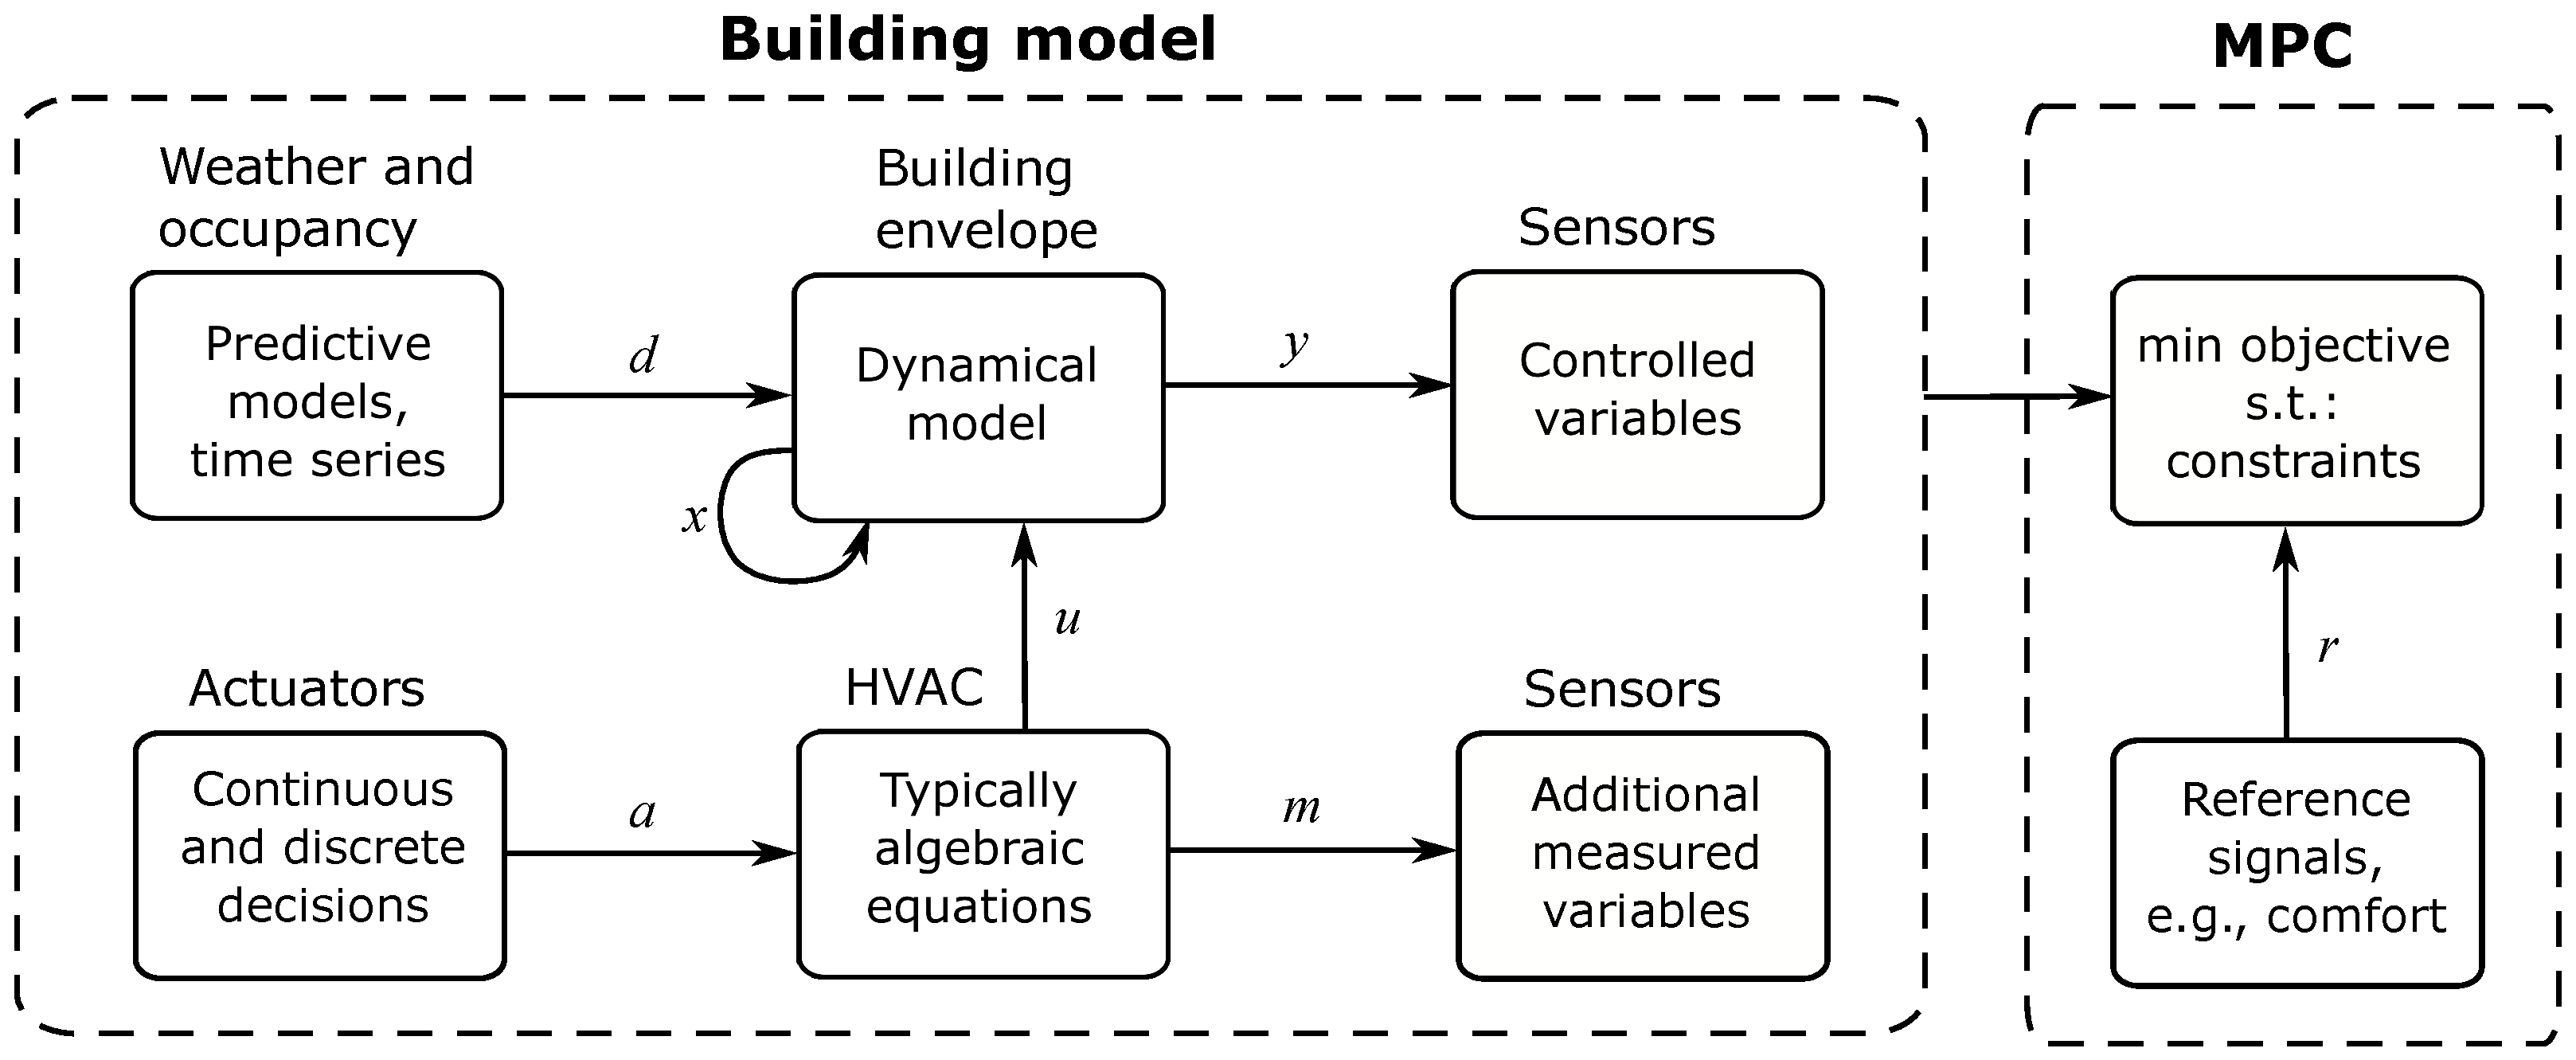
\includegraphics[width=0.70 \textwidth]{fig/Building_model_MPC.eps}
\caption{General structure of the building model with MPC.}
\label{fig:Building_model}
\end{figure}

The general MPC formulation can be cast as an optimal control problem (OCP) in discrete time:
\begin{subequations}
	\label{eq:mpc_general_formal}
	\begin{align}
	\min_{u_0, \ldots, u_{N-1}} & \ell_N(x_N) + \sum_{k=0}^{N-1} \ell_k(x_k, y_k, u_k, r_k, s_k) &
	\label{eq:mpc_general_formal:cost}\\
	\text{s.t.} \ & x_{k+1} = f(x_k, u_k, d_k),  & k \in \mathbb{N}_{0}^{N-1} & \label{eq:mpc_general_formal:xp} \\
	& y_{k} = g(x_k, u_k, d_k),  & k \in \mathbb{N}_{0}^{N-1} & \label{eq:mpc_general_formal:yp} \\
    &  u_{k} = f_{\text{HVAC}}(a_k,m_k),  & k \in \mathbb{N}_{0}^{N-1} & \label{eq:mpc_general_formal:u} \\
	& s_{k} = h(x_k, y_k, u_k, r_k),  & k \in \mathbb{N}_{0}^{N-1} & \label{eq:mpc_general_formal:s} \\
	&  x_{k} \in \mathcal{X},  & k \in \mathbb{N}_{0}^{N-1}   \label{eq:mpc_general_formal:xb}\\
	& u_{k} \in \mathcal{U}, & k \in \mathbb{N}_{0}^{N-1} 
	\label{eq:mpc_general_formal:ub}\\
    & a_{k} \in \mathcal{A}, & k \in \mathbb{N}_{0}^{N-1} 
	\label{eq:mpc_general_formal:ab}\\
	& s_{k} \in \mathcal{S}, & k \in \mathbb{N}_{0}^{N-1} 
	\label{eq:mpc_general_formal:sb}\\
	%   & \underline{x} \le x_k \le \overline{x}, \label{eq:mpc_general_formal:xb}\\
	%   & \underline{u} \le u_k \le \overline{u}, \label{eq:mpc_general_formal:ub}\\
    & d_k = d(t + k T_s),  & k \in \mathbb{N}_{0}^{N-1} \label{eq:mpc_general_formal:d0} \\
    & r_k = r(t + k T_s),  & k \in \mathbb{N}_{0}^{N-1} \label{eq:mpc_general_formal:r0} \\
	& x_0 = x(t),\label{eq:mpc_general_formal:x0} 
	\end{align}
\end{subequations}
where $x_k \in \mathbb{R}^{n_x}$, $y_k \in \mathbb{R}^{n_y}$, $u_k \in \mathbb{R}^{n_u}$, $a_k \in \mathbb{R}^{n_a}$,
$m_k \in \mathbb{R}^{n_m}$, $d_k \in \mathbb{R}^{n_d}$, $r_k \in \mathbb{R}^{n_r}$ and $s_k \in \mathbb{R}^{n_s}$ denote the values of states, outputs, envelope inputs, HVAC actuators, additional measured variables, disturbances, reference signals and slack variables respectively, at the $k$-th step of the prediction horizon $N$ with a sampling time $T_s$. 
Where $n_{\star}$ denotes the dimensionality of associated variable $\star$.


The objective function is given by~\eqref{eq:mpc_general_formal:cost} where   $\ell_N(x_N)$  represents the terminal penalty, while $\ell_k(x_k,y_k,u_k,r_k,s_k)$  is called a stage cost and its
purpose is to assign a cost to a particular choice of $x_k$, $y_k$, $u_k$, $r_k$ and $s_k$. For most of the building control applications the terminal penalty is omitted.
The predictions of the state values are obtained from the state update equation~\eqref{eq:mpc_general_formal:xp}, while values of the predicted outputs are given by the output equation~\eqref{eq:mpc_general_formal:yp}.
{\color{blue} 
The building envelope inputs are given by the HVAC model~\eqref{eq:mpc_general_formal:u}. }
Slack variables are defined as additional constraints~\eqref{eq:mpc_general_formal:s}, they ususally represent algebraic relations of state, output, or input variables.
% 
States, envelope inputs, actuators, and slack variables are subject to
constraints~\eqref{eq:mpc_general_formal:xb},~\eqref{eq:mpc_general_formal:ub},~\eqref{eq:mpc_general_formal:ab}, and~\eqref{eq:mpc_general_formal:sb},
where sets  $\mathcal{X}$, $\mathcal{U}$, $\mathcal{A}$, and $\mathcal{S}$ represent feasible subset of $\mathbb{R}^{n}$. 
% 
The initial conditions for the state variables are given by~\eqref{eq:mpc_general_formal:x0}, which are either  measured or estimated. 
Eq.~\eqref{eq:mpc_general_formal:d0} and~\eqref{eq:mpc_general_formal:r0} represent initialization of the disturbances and references  for the whole prediction horizon, obtained as a forecast.
% 
For the sake of generality we denote by $\xi$ the vector that encapsulates all initial conditions of~\eqref{eq:mpc_general_formal}, i.e. the current states $x(t)$, current and future disturbance variables $d(t), \ldots, d(t+N T_s)$, and possibly parameters such as comfort boundaries or reference signals which depend on the specific formulation.
The parameter $T_s$ here represents the sampling time.
Compression of all initial conditions into single vector $\xi$ is convenient for 
compact  representation of MPC feedback law in the form $U = f_{MPC}(\xi)$,
where $U = \begin{bmatrix} u_0 & u_1 & \cdots & u_{N-1} \end{bmatrix} $ is the vector of computed optimal control actions obtained as a solution of the problem~\eqref{eq:mpc_general_formal}.



\section{MPC FORMULATION IN BUILDINGS: GRANTING A PHYSICAL MEANING }

In Section~\ref{sec:control_notation} the abstract MPC formulation has been defined, now physical meaning and ranges of variables and parameters have to be specified.
% 
For the sake of clarity, we make a distinction between the meaning of variable and parameter in this document.
Variable represents a value which is computed by or is dynamically influencing the model equations~\eqref{eq:mpc_general_formal:xp} and~\eqref{eq:mpc_general_formal:yp}. For this reason, we will denote the measured disturbances such as weather forecast a variable.
Parameter on the other hand is a value which is not involved in model equations in a dynamical vay~\eqref{eq:mpc_general_formal:xp} and~\eqref{eq:mpc_general_formal:yp}. Parameters can be
 either set up by the engineer (e.g., prediction horizon $N$, objective weights $Q_{\star}$), or can be known a priory during the design process (e.g., specific  heat capacity $c_p$), or even continuously measured as time-varying signals (e.g., coefficient of performance $COP$, or price factor $p$).
The slack variables $s$, are labeled as variables because they are computed within MPC and usually depend on model dynamics.
% However, slacks $s$ they usually represent violations of particular constraints, hence they are only indirectly associated with physical domain variables via these constraints.
% For this reason to simplify the Tab.~\ref{tab:mpc_form:translation} by avoiding introduction of the auxiliary physical domain variables associated with slack variables (e.g., thermal discomfort) we chose to label the slack variables $s$ as parameters.

Table~\ref{tab:mpc_form:translation} summarizes the most common
variables used in building control and maps them with the abstract
notation from the control engineering notation presented in previous section. 
Because these variables are usually vectors, we indicate the
$i$-th element of the vector variable via supercsript $i$,
for instance the operative temperature in the $i$-th zone is denoted as $T_z^i$.
Please note that presented mapping of  variables from physical domain to abstract domain generalizes most common cases found in the literature. However, less common 
but technically feasible mapping can be applied in some specific cases, e.g. treating envelope temperatures as  disturbance signals.


An overview of the most common modifying and bounding parameters in building control together with their associated variables is presented in Table~\ref{tab:mpc_form:parameters:modifiers} and Table~\ref{tab:mpc_form:parameters:bounds}, respectively.
These parameters can be treated either as constant numerical  or time-varying values. For example, in the latter case the parameters can represent reference $r$ within the MPC formulation.




Table~\ref{tab:mpc_form:objectives} recaps the most common objectives used 
in the MPC formulation. These objectives can be combined in a multi-objective function. 
% 
Since the main objective of building control is the maximization of occupants comfort while using as little resources as possible,
usually two conflicting terms are found: an energy minimization term
and a comfort maximization term.  
% 
Eq.~\eqref{eq:mpc:objective:cost1} is an example of such
 multi-objective function,
where $||{Q_{\text{s}} s_{k}}||_2^2$ represents an arbitrary discomfort term in the form of the weighted squared 2-norm of the slack variables, and ${Q_{\text{u}} u_{k}}$ stands for the weighted linear energy term. The matrices $Q_{\text{s}}$ and $Q_{\text{u}}$ here stand for the weighting factors.
\begin{equation}
\min_{u_0, \ldots, u_{N-1}}  
\sum_{k=0}^{N-1} (||{Q_{\text{s}} s_{k} }||_2^2
+ {Q_{\text{u}}  u_{k}}) \label{eq:mpc:objective:cost1}
\end{equation}
% 
 
The energy used by the building stands for the sum of the energy used by each HVAC component $Q^i_{\text{HVAC}}$.
Generally, the power $P^i_{\text{HVAC}}$ of $i$-th HVAC component can be calculated as the time integral of the
ratio between the thermal power that it delivers $Q^i_{\text{HVAC}}$ and its efficiency $COP^i, EER^i$ or $\eta^i$. 
These efficiencies are parameters that can be considered either constant or variable
as a function of the inputs, states and disturbances.
The energy use
minimization function can be further transformed to monetary cost  using a price factor  $p^i$, which can be added to the formulation 
as a time-varying (in electric-based components), constant (in fuel-based components) or even negative 
(renewable-based components that inject energy into the grid) parameter.
The emission factor $e^i$ converts the energy used into the associated $CO_2$ emissions 
for the $i$-th component which can be variable for electric-based components,
constant for fuel-based components and zero for renewable-based components.
The renewable energy sources (RES) share $RES^i$ represents the fraction of renewable
energy coming from the  $i$-th component and depends on the RES share of the grid for
electric-based components. The share is zero for fuel-based ones and for
renewable-based components the share would be 100\%.
% 
The balance between the different objectives is typically adjusted
by means of weighting factors $Q_{\star}$ to give more or less priority to the associated objective term $\ell({\star})$ for a particular variable $\star$. For example the penalization on control inputs $u$ can be by denoted by a weighting term $Q_{u}$.

In general, there are two types of constraints:
inequality (control inputs range, comfort zones, etc.) and equality 
(building model dynamics, rate limits, etc.) constraints.
A recap of the most common constraints in building control can be found in
Table \ref{tab:mpc_form:constraints}.
The constraints which satisfaction is mandatory are called 
\textit{hard constraints}. For example, hard control action
bounds define the minumum $\underline{u}_k$ and maximum $\overline{u}_k$ allowed values for the contol variables.
 On the other hand, the constraints which can 
be violated are known as \textit{soft constraints}. They are usually relaxed
by slack variables $s_k$ that are added to and
penalized in the objective function (see comfort objective in Table
\ref{tab:mpc_form:objectives} and soft inequality constraints in Table \ref{tab:mpc_form:constraints}), trying to keep them within the bounds set. 
For example the thermal discomfort is typically evaluated via a slack variable $s_k$ which denotes the violation of a thermal comfort zone associated with zone operative temperature $T_z$.
All constraints can be time-varying.

% TODO: Q_i is conflicting notation with weights, keep using Q_{HVAC}^i
\begin{table}[ht]
	% Suppressing floating placement of tables/figures in LaTeX is generally deprecated. 
	{\color{blue} 
	\centering
	\caption{MPC variables notation and translation between physical and abstract domain.}
	\label{tab:mpc_form:translation}
	\begin{adjustwidth}{-1cm}{}
	\begin{tabular}{l|c|l|ccccccc}
		\toprule
        \multicolumn{3}{l}{\textbf{Physical domain}} &  \multicolumn{6}{r}{\textbf{Abstract domain}} \\
		\toprule
		\textbf{Variables} & \textbf{Symbol} & \textbf{Description} & \textbf{$x$} & \textbf{$y$} & \textbf{$m$} & \textbf{$a$} & \textbf{$u$} & \textbf{$d$}   & \textbf{$s$} \\ 
		\midrule
		\multirow{8}{*}{\textbf{Temperatures [\SI{}{\celsius}]}} & $T$ & Envelope temperatures (wall, concrete, glazing...) & $\bullet$ & -  & - & - & -& -& -\\ 
		& $T_{\text{z}}$ & Zone operative temperatures  & - & $\bullet$ & -  & - & -& -& -\\
		& $T_{\text{sup}}^{\text{HVAC}}$ & Supply temperatures  of  HVAC  &  - & - & $\bullet$ & -  & -& -& -\\
		& $T_{\text{ret}}^{\text{HVAC}}$ & Return temperatures  of  HVAC  &  - & - & $\bullet$ & - & -& -& - \\
		& $T^{\text{HVAC}}_{\text{sp}}$ & Set-points of HVAC supply temperatures    &  - & - & - & $\bullet$ & - & -& -\\
		& $T_\text{e}$ & Ambient temperature &  - & -& -& - & - & $\bullet$ & -\\
		& $T_\text{b}$ & Borefield wall temperature & $\bullet$ & - & - & -  & - & - & - \\
			& $T_\text{g}$ & Borefield  ground temperatures & $\bullet$ & - & - & -  & - & - & -\\
% 			& $T_{\text{sg,}i}$ & Borefield surrounding ground temperature at distance $i$ & $\bullet$ & - & - & - \\
		\midrule
		\multirow{3}{*}{\textbf{Thermal energy $[J]$}} 
		% 		& $Q$ & Total heat flow  of HVAC components & - & - & $\bullet$ & -  \\
		& $Q_{\text{HVAC}}$ & Thermal energy of the HVAC components  & - & -&  $\bullet$ & - & - &- & - \\
		& $Q_{\text{b}}$ & \makecell[l]{Thermal energy injected/extracted \\ into/from the borefield} & - & - & $\bullet$ & - & - & - & -  \\
		\midrule
		\multirow{5}{*}{\textbf{Thermal power $[W]$}} 
% 		& $Q$ & Total heat flow  of HVAC components & - & - & $\bullet$ & -  \\
		& $\dot{Q}_{\text{HVAC}}$ & Thermal power of  HVAC components  & - & -& -& - &  $\bullet$ &- & - \\
		& $\dot{Q}_{\text{rad}}$ & Solar radiation & - & - & - & - & - & $\bullet$ & - \\
		& $\dot{Q}_{\text{occ}}$ & Occupancy internal gains  & - & - & - & - & - & $\bullet$ & - \\
		& $\dot{Q}_{\text{lig}}$ & Lighting internal gains & - & - & - & -  & $\bullet$ & $\bullet$ & -  \\
		& $\dot{Q}_{\text{app}}$ & Appliances internal gains & - & - & - & -  & $\bullet$ & $\bullet$ & -  \\
		\midrule
		\multirow{3}{*}{\textbf{Electrical energy $[J]$}} 
		% 	& $P$ & Total power  of HVAC components & - & - & $\bullet$ & - \\
		& $E_{\text{HVAC}}$ & Electrical energy used by HVAC components & - & - &  $\bullet$ &-  & -  & -  & - \\
		& $E_{\text{lig}}$ & Electrical energy used by lighting & - & - & $\bullet$  & -  & -  & -  & -  \\
		& $E_{\text{app}}$ & Electrical energy used by appliances & - & - & $\bullet$  & -  & -  & -  & - \\
		\midrule
		\multirow{3}{*}{\textbf{Electrical power $[W]$}} 
% 	& $P$ & Total power  of HVAC components & - & - & $\bullet$ & - \\
		& $P_{\text{HVAC}}$ & Power of HVAC components & - & -  &  $\bullet$ &-  & -& -& -\\
		& $P_{\text{lig}}$ & Lighting power & - & -  &  $\bullet$ &-  & -& -& -\\
		& $P_{\text{app}}$ & Appliances power & - & -  &  $\bullet$ &-  & -& -& -\\
\midrule
		\multirow{1}{*}{\textbf{Mass flows $[kg/s]$}} &
		$\dot{m}_{\text{HVAC}}$ & Water/air mass flow rates of HVAC & - & - & $\bullet$ &  $\bullet$ & -  & -  & -  \\
% 		& $\dot{m}_{\text{air}}$ & Air mass flow & - & - & $\bullet$ &  $\bullet$  & -  & -  & - \\
		\midrule
		\multirow{5}{*}{\textbf{\shortstack[l]{Component signals }}} 
% 		& $T^{set}_{\text{sup}}$ & Supply system set-points & - & - & $\bullet$ & - \\
% 		& $T^{set}_{z}$ & Zone set-point & - & - & $\bullet$ & - \\
		& $x_{\text{HVAC}}$ & \makecell[l]{ON/OFF/Modulated signal of \\ HVAC components $[\{0,1\},\%]$ }& - & - & -  & $\bullet$ & -  & -  & - \\
		& $\Delta p$ & Pump/fan difference pressure $[kPa]$ & - & - & -  & $\bullet$ & -  & -  & - \\
		& $x_{\text{mov}}$ & Pump/fan speed signal $[\%,kPa]$ & - & - & -  & $\bullet$ & -  & -  & - \\
		& $x_{\text{val}}$ & Valve positions $[\%]$  & - & - & -  & $\bullet$ & -  & -  & - \\
		& $x_{\text{dam}}$ & Damper positions $[\%]$ & - & - & -  & $\bullet$ & -  & -  & - \\
		\midrule
		\multirow{4}{*}{\textbf{\shortstack[l]{Indoor Environmental \\ Quality (IEQ)}}} &
		$PMV$ & Predicted mean vote $[-]$ & - & $\bullet$ & - & - & -& -& -\\
		& $CO_2$ & $CO_2$ concentration in air $[ppm]$ & - & $\bullet$ & - & - & -& -& -\\
		& $\phi$ & Relative humidity  $[\%]$ & - & $\bullet$ & - & - & -& -& -\\
		& $E_{\text{v}}$ & Illuminance $[lx]$ & - & $\bullet$ & - & - & -& -& -\\
			\midrule
		\multirow{6}{*}{\textbf{Constraints violations}} 
		 &
		$s^{\star}$ & Violations of constraints on variable $\star$ [-] & - &- &- & - & - & - & $\bullet$ \\
		&
		$s^{T_{\text{z}}}$ & Violations of thermal comfort zones [\SI{}{\celsius}] & - &- &- & - & - & - & $\bullet$ \\
		&
		$s^{PMV}$ & Violations of PMV zones [-] & - &- &- & - & - & - & $\bullet$ \\
		&
		$s^{CO_2}$ & Violations of $CO_2$  concentration limits $[ppm]$ & - &- &- & - & - & - & $\bullet$ \\
		&
		$s^{\phi}$ & Violations of relative humidity  limits $[\%]$ & - &- &- & - & - & - & $\bullet$ \\
		&
		$s^{E_{\text{v}}}$ & Violations of illuminance  limits $[lx]$ & - &- &- & - & - & - & $\bullet$ \\
		\bottomrule 
	\end{tabular}
	 \end{adjustwidth}
	 }
\end{table} 


\renewcommand{\arraystretch}{2}
\begin{table}[ht]
	% Suppressing floating placement of tables/figures in LaTeX is generally deprecated. 
	\centering
	\caption{MPC formulation parameters - modifiers and tuning parameters.}
	\label{tab:mpc_form:parameters:modifiers}
	\begin{tabular}{l|c|l|c}
		\toprule
		\textbf{Energy efficiencies}  & \textbf{Symbol} &  \textbf{Description} & \textbf{Associated variables} \\
		\midrule
		\makecell[l]{Coefficient of \\ performance} & $COP^i$ &  \makecell[l]{Coefficient of performance \\ of heat pump $i$} & $T_{\text{sup}}^{\text{HVAC}}, \dot{Q}^i_{\text{HVAC}}, P^i_{\text{HVAC}}$ \\
		\makecell[l]{Energy efficiency \\ ratio} & $EER^i$ & \makecell[l]{Cooling efficiency of \\ air conditioning system $i$} & $T_{\text{sup}}^{\text{HVAC}}, \dot{Q}^i_{\text{HVAC}}, P^i_{\text{HVAC}}$ \\
		Efficiency & $\eta^i$ & \makecell[l]{Efficiency of other  $i$-th system} & $T_{\text{sup}}^{\text{HVAC}}, \dot{Q}^i_{\text{HVAC}}, P^i_{\text{HVAC}}$ \\
		\makecell[l]{Seasonal coefficient of \\ performance} & $SCOP^i$ &  \makecell[l]{Seasonal coefficient of performance \\ of heat pump $i$} & $T_{\text{sup}}^{\text{HVAC}}, Q^i_{\text{HVAC}}, E^i_{\text{HVAC}}$ \\
		\makecell[l]{Seasonal energy efficiency \\ ratio} & $SEER^i$ & \makecell[l]{Seasonal cooling efficiency of \\ air conditioning system $i$} & $T_{\text{sup}}^{\text{HVAC}}, Q^i_{\text{HVAC}}, E^i_{\text{HVAC}}$  \\
		\midrule
		\textbf{Other energy factors}  & \textbf{Symbol} &  \textbf{Description} & \textbf{Associated variables} \\
		\midrule
		Price factor & $p^i$ &  \makecell[l]{Conversion factor from energy \\ to monetary cost of component $i$} & $Q^i_{\text{HVAC}}$ \\
		Emission factor & $e^i$ & \makecell[l]{Conversion factor from energy \\ to $CO_2$ emissions of component $i$} & $Q^i_{\text{HVAC}}$ \\
		RES factor & $RES^i$ & \makecell[l]{Share of renewable energy of \\ the considered component $i$} & $Q^i_{\text{HVAC}}$ \\
			\midrule
		\textbf{Heat flow parameters}  & \textbf{Symbol} &  \textbf{Description} & \textbf{Associated variables} \\
		\midrule
		Specific heat capacity & $c_p^i$ & \makecell[l]{Specific heat capacity of \\ $i$-th medium} & $T_{\text{sup}}^{\text{HVAC}}, T_{\text{ret}}^{\text{HVAC}}, \dot{m}_{\text{wat}}, \dot{m}_{\text{air}}, \dot{Q}^i_{\text{HVAC}}$ \\
		\midrule
		\textbf{Tuning parameters}  & \textbf{Symbol} &  \textbf{Description} & \textbf{Associated variables} \\
		\midrule
%         \makecell[l]{Slack variable} & $s$ &  \makecell[l]{Used to soften the constraints, usually \\ for the given comfort requirement} 
% 		&  all \\
		\makecell[l]{Weighting factor} & $Q_{\star}$ &  \makecell[l]{Weighting for the particular term \\ in the objective function} & all \\
		\makecell[l]{Sampling time} & $T_{s}$ &  \makecell[l]{Time-step used in the \\ optimization problem} & all  \\
		\makecell[l]{Dimensionality quantifier} & $n_{\star}$ &  \makecell[l]{Cardinality of the vector elements} & all \\
		\bottomrule 
	\end{tabular}
\end{table}



\renewcommand{\arraystretch}{2}
\begin{table}[ht]
	% Suppressing floating placement of tables/figures in LaTeX is generally deprecated. 
	\centering
	\caption{MPC formulation parameters - bounds and references $r$.}
	\label{tab:mpc_form:parameters:bounds}
		\begin{adjustwidth}{-1.5cm}{}
	\begin{tabular}{l|c|l|c}
		\toprule
		\textbf{Comfort bounds $r$}  & \textbf{Symbol} &  \textbf{Description} & \textbf{Associated variables} \\
		\midrule
		Temperature & $\underline{T_{\text{z}}},\overline{T_{\text{z}}}$ & \makecell[l]{Zone operative temperature  \\ comfort bounds } & $T_{\text{z}}$ \\
		$CO_2$ concentration & $\underline{CO_2},\overline{CO_2}$ & \makecell[l]{$CO_2$ concentration comfort \\ bounds} & $CO_{2}$ \\
		Predicted mean vote & $\underline{PMV},\overline{PMV}$ &  \makecell[l]{Predicted mean vote comfort \\ bounds} & $PMV$ \\
		Humidity & $\underline{\phi},\overline{\phi}$ &  Humidity comfort bounds & $\phi$  \\
		Illuminance & $\underline{E_{\text{v}}},\overline{E_{\text{v}}}$ & Illuminance comfort bounds & $E_{\text{v}}$  \\
		\bottomrule 
		\textbf{Component limitations}  & \textbf{Symbol} &  \textbf{Description} & \textbf{Associated variables} \\
		\midrule
		Thermal power limit & $\underline{\dot{Q}^i_{\text{HVAC}}},\overline{\dot{Q}^i_{\text{HVAC}}}$ & \makecell[l]{Min/max thermal power of \\ the $i$-th HVAC component} & $Q^i_{\text{HVAC}}$ \\
		\makecell[l]{Rate of change of\\ thermal power rate}  & $\underline{\Delta \dot{Q}^i_{\text{HVAC}}},\overline{\Delta \dot{Q}^i_{\text{HVAC}}}$ & \makecell[l]{Min/max rate of change of  thermal  \\ power  of the  $i$-th HVAC component} & $Q^i_{\text{HVAC}}$ \\
		\makecell[l]{Pump difference\\ pressure limit}   & $\underline{\Delta p^i},\overline{\Delta p^i}$ & \makecell[l]{Min/max diff. pressure \\  of the  $i$-th fan/pump} & $\Delta p^i$ \\
		\makecell[l]{Rate of change of\\ pump difference pressure}   & $\underline{\Delta\Delta p^i},\overline{\Delta\Delta p^i}$ & \makecell[l]{Min/max rate of  change of \\ diff. pressure of the  $i$-th fan/pump} & $\Delta p^i$ \\
		Pump speed limit & $\underline{ x^i_{\text{mov}}},\overline{ x^i_{\text{mov}}}$ & \makecell[l]{Min/max  speed of \\  the  $i$-th fan/pump} & $x^i_{\text{mov}}$ \\
		\makecell[l]{Rate of change of\\ pump speed}  & $\underline{\Delta x^i_{\text{mov}}},\overline{\Delta x^i_{\text{mov}}}$ & \makecell[l]{Min/max rate of  change of \\ speed of the  $i$-th fan/pump} & $x^i_{\text{mov}}$ \\
		Valve position limits & $\underline{ x^i_{\text{val}}},\overline{ x^i_{\text{val}}}$ & \makecell[l]{Min/max position of \\  the  $i$-th valve} & $x^i_{\text{val}}$ \\
		\makecell[l]{Rate of change of\\ valve position}  & $\underline{\Delta x^i_{\text{val}}},\overline{\Delta x^i_{\text{val}}}$ & \makecell[l]{Min/max change of \\ position of the  $i$-th valve} & $x^i_{\text{val}}$ \\
		Damper position limits& $\underline{ x^i_{\text{dam}}},\overline{ x^i_{\text{dam}}}$ & \makecell[l]{Min/max position of \\  the  $i$-th damper} & $x^i_{\text{dam}}$ \\
		\makecell[l]{Rate of change of\\ damper position} 
		& $\underline{\Delta x^i_{\text{dam}}},\overline{\Delta x^i_{\text{dam}}}$ & \makecell[l]{Min/max rate of  change of \\ position of the  $i$-th damper} & $x^i_{\text{dam}}$ \\
		\bottomrule 
	\end{tabular}
	\end{adjustwidth}
\end{table}

% TODO: add dimensions to variables and parameters?

% TODO: add definition and use of mathematical norms, 1,2,inf
\renewcommand{\arraystretch}{2.5}
\begin{table}[ht]
	% Suppressing floating placement of tables/figures in LaTeX is generally deprecated. 
	\centering
	\caption{Additive terms $\star$ of MPC objective $\min  \sum_{k=0}^{N-1} \star$.}
	\label{tab:mpc_form:objectives}
	\begin{tabular}{l|lll}
		\toprule
		\textbf{Linguistic objective}  &  \multicolumn{3}{c}{\textbf{MPC formulation}} \\
		& Class &  Control notation &  Physical notation \\
		\midrule
% 		\textbf{Linguistic objective}  & \textbf{MPC formulation} \\
		\midrule
		Minimize energy use & linear  &  $ \sum_{i=1}^{n_u} u^{i}_{k}$ &  $  \sum_{i=1}^{n_{\dot{Q}_{\text{HVAC}}}} \dot{Q}^{i}_{\text{HVAC},k}$ \\
		Minimize power use & linear  &  $  \sum_{i=1}^{n_u} \dfrac{u^{i}_{k}}{\eta_k^i}$ &  $  \sum_{i=1}^{n_{\dot{Q}_{\text{HVAC}}}} \dfrac{\dot{Q}^{i}_{\text{HVAC},k}}{\eta_k^i}$ \\
		Minimize cost & linear &  $  \sum_{i=1}^{n_u} p_k^i \dfrac{u^{i}_{k}}{\eta_k^i}$ & $  \sum_{i=1}^{n_{\dot{Q}_{\text{HVAC}}}} p_k^i \dfrac{\dot{Q}^{i}_{\text{HVAC},k}}{\eta_k^i}$  \\
		Minimize $CO_2$ emissions & linear &  $  \sum_{i=1}^{n_u} e_k^i \dfrac{u^{i}_{k}}{\eta_k^i}$ &  $ \sum_{i=1}^{n_{\dot{Q}_{\text{HVAC}}}}  e_k^i \dfrac{\dot{Q}^{i}_{\text{HVAC},k}}{\eta_k^i}$  \\
		Maximise RES &  linear &  $  \sum_{i=1}^{n_u} (1-RES_k^i) \dfrac{u^{i}_{k}}{\eta_k^i}$ & $ \sum_{i=1}^{n_{\dot{Q}_{\text{HVAC}}}} (1-RES_k^i) \dfrac{\dot{Q}^{i}_{\text{HVAC},k}}{\eta_k^i}$  \\
			Minimize discomfort &  quadratic &  $  ||s_k||^2_2$ &  $ ||s^{T_{\text{z}}}_k||^2_2$  \\
% 		Minimize discomfort &  quadratic &  $ \sum_{i=1}^{n_s} ||s^i_k||^2_2$ &  $ \sum_{i=1}^{n_{s^{T_{\text{z}}}}} ||s^{T_{\text{z}},i}_k||^2_2$  \\
		Flexibility &  TBD & TBD  & TBD \\
		\bottomrule 
	\end{tabular}
\end{table}

\renewcommand{\arraystretch}{2.5}
\begin{table}[ht]
	% Suppressing floating placement of tables/figures in LaTeX is generally deprecated. 
	\centering
	\caption{MPC formulation constraints.}
	\label{tab:mpc_form:constraints}
	\begin{adjustwidth}{-1cm}{}
	\begin{tabular}{l|lll}
		\toprule
		\textbf{Linguistic constraint}  &  \multicolumn{3}{c}{\textbf{MPC formulation}} \\
		& Class &  Control notation &  Physical notation \\
		\midrule
		Envelope dynamics & hard equality & $ x_{k+1} = f(x_k,u_k,d_k) $  & $ T_{k+1} = f(T_k,\dot{Q}_{\text{HVAC},k},T_{\text{e},k},\dot{Q}_{\text{rad},k},\dot{Q}_{\text{occ},k},\dot{Q}_{\text{lig},k}) $ \\ 
		{\color{blue} HVAC model } & hard equality & $ u_{k} = f_{\text{HVAC}}(a_k,m_k) $  & $ \dot{Q}_{\text{HVAC},k} = f_{\text{HVAC}}(\dot{m}_{\text{HVAC}}, T_{\text{sup}}^{\text{HVAC}},T_{\text{ret}}^{\text{HVAC}},P_{\text{HVAC}}) $ \\ 
		Component limitations & hard inequality & $ \underline{u}_k \le u_k \le \overline{u}_k  $  & $ \underline{\dot{Q}_{\text{HVAC}}}_k  \le \dot{Q}_{\text{HVAC},k}  \le \overline{\dot{Q}_{\text{HVAC}}}_k  $ \\ 
		Component difference & hard equality & $\Delta u_k = u_{k-1} - u_k $  & $\Delta \dot{Q}_{\text{HVAC},k} = \dot{Q}_{\text{HVAC},k-1} - \dot{Q}_{\text{HVAC},k} $  \\ 
		Component rate of change & hard inequality & $ \underline{\Delta u}_k   \le \Delta u_k  \le \overline{\Delta u}_k  $ & $ \underline{\Delta \dot{Q}_{\text{HVAC}}}_k   \le \Delta \dot{Q}_{\text{HVAC},k}  \le \overline{\Delta \dot{Q}_{\text{HVAC}}}_k  $ \\ 
		Temperature comfort zone & soft inequality & $ \underline{y}_k - s_k \le y_k \le \overline{y}_k + s_k $  & $ \underline{T_{\text{z}}}_k - s^{T_{\text{z}}}_{k} \le T_{\text{z}} \le \overline{T_{\text{z}}}_k + s^{T_{\text{z}}}_{k} $ \\
		$CO_2$ concentration & soft inequality & $ \underline{y}_k - s_k \le y_k \le \overline{y}_k + s_k $ & $ \underline{{CO_2}}_k - s^{CO_2}_k \le CO_2 \le \overline{{CO_2}}_k + s^{CO_2}_k $  \\
		Predicted mean vote &  soft inequality & $ \underline{y}_k - s_k \le y_k \le \overline{y}_k + s_k $ & $ \underline{PMV}_k - s^{PMV}_k \le PMV \le \overline{PMV}_k + s^{PMV}_k $  \\
		Humidity & soft inequality & $ \underline{y}_k - s_k \le y_k \le \overline{y}_k + s_k $ & $ \underline{\phi}_k - s^{\phi}_k \le \phi \le \overline{\phi}_k + s^{\phi}_k $  \\
		Illuminance & soft inequality & $ \underline{y}_k - s_k \le y_k \le \overline{y}_k + s_k $ & $ \underline{{E_\text{v}}}_k - s^{E_\text{v}}_k \le E_\text{v} \le \overline{{E_\text{v}}}_k + s^{E_\text{v}}_k $  \\
		\bottomrule 
	\end{tabular}
	\end{adjustwidth}
\end{table}


%\bibliographystyle{apacite}
%\bibliography{template}
%\vspace{24pt}


\section*{ACKNOWLEDGMENTS}

This work emerged from the IBPSA Project 1, an international project conducted under the umbrella of the International Building Performance Simulation Association (IBPSA). Project 1 will develop and demonstrate a BIM/GIS and Modelica Framework for building and community energy system design and operation.

The authors acknowledge the financial support by the European Union through  the EU-H2020-GEOT\euro CH 
project ‘Geothermal Technology for \euro conomic Cooling and Heating’ 
and within the H2020-EE-2016-RIA-IA programme for the project ‘Model Predictive Control and Innovative System Integration of GEOTABS;-) 
in Hybrid Low Grade Thermal Energy Systems - Hybrid MPC GEOTABS’ (grant number 723649 - MPC-; GT). 

\end{document}
